% Created 2024-09-29 Sun 18:03
% Intended LaTeX compiler: pdflatex
\documentclass[11pt]{article}
\usepackage[utf8]{inputenc}
\usepackage[T1]{fontenc}
\usepackage{graphicx}
\usepackage{longtable}
\usepackage{wrapfig}
\usepackage{rotating}
\usepackage[normalem]{ulem}
\usepackage{amsmath}
\usepackage{amssymb}
\usepackage{capt-of}
\usepackage{hyperref}
\usepackage{minted}
\usepackage[a4paper, margin=2.5cm]{geometry}
\usepackage{minted}
\usepackage{fontspec}
\setmonofont{Iosevka}
\setminted{fontsize=\small, frame=single, breaklines=true}
\usemintedstyle{emacs}
\author{Baley Eccles - 652137}
\date{\textit{{[}2024-09-17 Tue 10:17]}}
\title{ENG231 - Electrical Machines And Transformers - Assesment 2 Lab 4}
\hypersetup{
 pdfauthor={Baley Eccles - 652137},
 pdftitle={ENG231 - Electrical Machines And Transformers - Assesment 2 Lab 4},
 pdfkeywords={},
 pdfsubject={},
 pdfcreator={Emacs 29.4 (Org mode 9.8)}, 
 pdflang={English}}
\begin{document}

\maketitle
\tableofcontents

\section{ENG231 - Electrical Machines And Transformers - Assesment 2 Lab 4}
\label{sec:orgce43c33}
\subsection{Name Plate}
\label{sec:org780c98c}
{[}Group] Report your transformer nameplate ratings
\begin{longtable}{|l|l|}
\hline
VA ratings & 500\\
\hline
\endfirsthead
\multicolumn{2}{l}{Continued from previous page} \\
\hline

VA ratings & 500 \\

\hline
\endhead
\hline\multicolumn{2}{r}{Continued on next page} \\
\endfoot
\endlastfoot
\hline
Primary voltage (\(V\)) & 240\\
\hline
Secondary voltage (\(V\)) & 115\\
\hline
Primary current (\(A\)) & 2.1\\
\hline
Secondary current (\(A\)) & 4.4\\
\hline
Turns ratio & 2.1\\
\hline
\end{longtable}
\subsection{DC Test}
\label{sec:org71add58}
{[}Group] Report your transformer DC test results, commenting on the relative resistances observed for each side of the transformer winding.
\begin{longtable}{|l|l|}
\hline
Primary resistance (\(R_{1dc}\)) (\(\Omega\)) & 1.5\\
\hline
\endfirsthead
\multicolumn{2}{l}{Continued from previous page} \\
\hline

Primary resistance (\(R_{1dc}\)) (\(\Omega\)) & 1.5 \\

\hline
\endhead
\hline\multicolumn{2}{r}{Continued on next page} \\
\endfoot
\endlastfoot
\hline
Secondary resistance (\(R_{2dc}\)) (\(\Omega\)) & 0.4\\
\hline
\end{longtable}
The primary side has a higher resistance than the secondary side, this is because the primary side has more turns. This will result in a longer wire and hence a larger resistance.\\
{[}Group] Calculate an ‘expected’ or ‘estimated’ total equivalent winding AC resistance Req as viewed from LV side and HV side of the transformer.
\begin{align*}
a&=2.1 \\
R_{eqHV}&=a^{2}R_2+R_1\\
R_{eqHV}&=3.264\Omega \\
R_{eqLV}&=a^{2}R_1+R_2\\
R_{eqLV}&=7.015\Omega \\
\end{align*}
\subsection{Open Circuit Test}
\label{sec:org8f46b7b}
\begin{longtable}{|l|l|l|l|l|l|}
\hline
 & Primary &  &  &  & Secondary\\
\hline
\endfirsthead
\multicolumn{6}{l}{Continued from previous page} \\
\hline

 & Primary &  &  &  & Secondary \\

\hline
\endhead
\hline\multicolumn{6}{r}{Continued on next page} \\
\endfoot
\endlastfoot
\hline
 & V1 & I1 & Poc & PF & V2\\
\hline
LV side open & 110 & 0.563 & 10.3 & 0.165 & 220\\
\hline
HV side open & 240 & 0.375 & 12.5 & 0.138 & 120\\
\hline
\end{longtable}
{[}Group] Calculate turns ratio for your transformer (a = N1 / N2) based on measured open-circuit voltages. Explain why there is a difference (if there is any difference) between your measurements and the nameplate voltages?
\begin{align*}
&\textrm{LV side open} & &\textrm{HV side open} \\
a&=\frac{V_{2}}{V_{1}} & a&=\frac{V_{2}}{V_{1}} \\
a&=2 & a&=2
\end{align*}
Both sides result is the same turns ratio. \\
{[}Group] Calculate power factor from voltage, current and power measurements and verify that it matches your measured value (from power analyser)
\begin{align*}
&\textrm{LV side open} & &\textrm{HV side open} \\
PF&=\frac{P_{oc}}{V_1I_1} & PF&=\frac{P_{oc}}{V_1I_1} \\
&=0.16631 & &= 0.13889
\end{align*}
The calculated power factor is very close to the measured power factor, which is to be expected. \\
{[}Group] Calculate the core resistance Rc1 and the magnetising reactance Xm1. (Do this now in the lab and check with the demonstrator that you have something reasonable before you continue)
\begin{align*}
&\textrm{LV side open} & &\textrm{HV side open} \\
R_{c1}&=\frac{V_1^2}{P_{oc}} & R_{c1}&=\frac{V_1^2}{P_{oc}} \\
&=1174.76\Omega & &=4680\Omega \\
X_{m1}&=\frac{V_1}{\sqrt{I_1^2+\left(\frac{V_1}{R_{c1}}\right)^2}} & X_{m1}&=\frac{V_1}{\sqrt{I_1^2+\left(\frac{V_1}{R_{c1}}\right)^2}} \\
&=192.73\Omega & &=633.92\Omega
\end{align*}

{[}Individual] Comment on the differences, if any, between supplying power and measuring from the HV side or the LV side \\
The LV side shows a higher power factor compared to the HV side. This means that the LV side consumes more power. This makes sense with the calculated resistances, the LV side has a higher resistance and hence a higher power draw. Although, this could also be due to the differences in input voltage during each test.

{[}Individual] Calculate the \% increase in current observed when voltage is increased by 20\% above rated voltage? Comment on your observations and discuss?
\begin{longtable}{|l|l|l|l|l|}
\hline
\(V_1\) (V) & \(I_1\) (A) & \(P_{oc}\) (W) & PF & \(V_2\) (V)\\
\hline
\endfirsthead
\multicolumn{5}{l}{Continued from previous page} \\
\hline

\(V_1\) (V) & \(I_1\) (A) & \(P_{oc}\) (W) & PF & \(V_2\) (V) \\

\hline
\endhead
\hline\multicolumn{5}{r}{Continued on next page} \\
\endfoot
\endlastfoot
\hline
138.25 & 1.28 & 18.4 & 0.102 & 275.4\\
\hline
\end{longtable}
Increase in current:
\begin{align*}
\%I_{increase}&=\frac{1.28-0.563}{0.563}\cdot 100\\
\%I_{increase}&=127.35\%
\end{align*}
This value shows that for a small increase in voltage we will get a disproportionally large increase in current. This implies a non-linear relationship between the current and voltage. Given that we are at the maximum rating for the transformer, we may be reaching the saturation region, this can be confirmed using the power factor, which is mostly reactive. This means that the energy from the increase in voltage is being used to magnetise the core, rather than transfer it to the other side. \\
{[}Individual] On the Power Analyser (still while operating at 20\% above rated voltage) observe transformer supply V and I waveforms. Include a sketch or image of a key waveform observed to help describe what you have observed and why? Does the waveform vary as supply voltage is varied? \\
Our team forgot to do this. However, we would expect to see the waveforms differ from usual operation. As shown, the transformer is being saturated, when this happens the magnetic flux in the core becomes distorted, which will effect the voltage and current waveforms. The current waveform will be more distorted than the voltage waveform, due to the introduction of a third harmonic, which will make the waveform less sinusoidal. These effects will be present in the voltage waveform, but less pronounced.
\begin{FIGURE}
\begin{figure}[H]
\centering
\includegraphics[width=.9\linewidth]{Screenshot 2024-09-29 at 12-13-26 crowhurst_basic_audio_vol2-125.gif (GIF Image 409 × 167 pixels).png}
\caption{Current and voltage waveform for a saturated transformer.}
\end{figure}
\end{FIGURE}
\subsection{Short Circus Test}
\label{sec:orgef630ea}
\begin{longtable}{|l|l|l|l|l|l|}
\hline
 & Primary &  &  &  & Secondary\\
\hline
\endfirsthead
\multicolumn{6}{l}{Continued from previous page} \\
\hline

 & Primary &  &  &  & Secondary \\

\hline
\endhead
\hline\multicolumn{6}{r}{Continued on next page} \\
\endfoot
\endlastfoot
\hline
 & V1 & I1 & Psc & PF & I2\\
\hline
LV side Short circuited & 7 & 1.76 & 10 & 0.863 & 3.5\\
\hline
\end{longtable}

{[}Group] Calculate \(R_{eq}\) \& \(X_{eq}\).
\begin{align*}
R_{eq}&=\frac{P_{sc}}{I_1^2} \\
&=3.228\Omega \\
X_{eq}&=\sqrt{\left(\frac{V_1}{I_1}\right)^2-R_{eq}^{2}} \\
&=5.123\Omega
\end{align*}

{[}Group] Calculate power factor from these values and verify your measured value.
\begin{align*}
PF&=\frac{P_{sc}}{V_1I_1} \\
&=0.81169
\end{align*}
The calculated power factor closely matches the measured one. \\
{[}Individual] Compare \(R_{eq}\) (equivalent winding AC resistance) to the DC resistance values measured earlier (you will need to refer them both to the same side). Why do you think there is a difference (if there is any)?
\(R_{dcTotal}=3.1\Omega\) and \(R_{eq}=3.228\Omega\), we can see that AC resistance is slightly larger than the DC resistance. This is because the AC resistance takes into account more effects that don't apply during DC, such as Eddy currents. \\
{[}Individual] Draw the full equivalent circuit for your transformer, labelling impedances with your determined transformer parameters
\begin{FIGURE}
\begin{figure}[H]
\centering
\includegraphics[width=.9\linewidth]{/home/Baley/UTAS/ENG231 - Electrical Machines And Transformers/Lab 4/Transformer.png}
\caption{Full equivalent circuit for our transformer.}
\end{figure}
\end{FIGURE}
\subsection{Performance Test / Full Load Test}
\label{sec:org948e2b6}
\begin{longtable}{|l|l|l|l|l|l|l|l|l|l|}
\hline
 & Load & 0ohm & 200ohm & 150ohm & 100ohm & 75ohm & 50ohm & 33ohm & 25ohm\\
\hline
\endfirsthead
\multicolumn{10}{l}{Continued from previous page} \\
\hline

 & Load & 0ohm & 200ohm & 150ohm & 100ohm & 75ohm & 50ohm & 33ohm & 25ohm \\

\hline
\endhead
\hline\multicolumn{10}{r}{Continued on next page} \\
\endfoot
\endlastfoot
\hline
Primary & V1 & 240 & 240 & 240 & 240 & 240 & 240 & 240 & 240\\
\hline
 & I1 & 0.375 & 0.495 & 0.56 & 0.71 & 0.88 & 1.2 & 1.75 & 2.28\\
\hline
 & P1 & 12 & 80 & 102 & 147 & 191 & 277 & 409 & 537\\
\hline
 & PF & 0.138 & 0.677 & 0.76 & 0.861 & 0.912 & 0.954 & 0.977 & 0.958\\
\hline
Secondary & V2 & 120 & 120 & 119 & 118 & 118 & 117 & 116 & 115\\
\hline
 & I2 & 0 & 0.56 & 0.753 & 1.12 & 1.5 & 2.2 & 3.3 & 4.4\\
\hline
 & P2 & 0 & 67 & 90 & 133 & 177 & 262 & 386 & 509\\
\hline
 & PF & NULL & 1 & 1 & 1 & 1 & 1 & 1 & 1\\
\hline
\% Voltage &  & 0 & 0 & 0.8403 & 1.694 & 1.695 & 2.564 & 3.448 & 4.347\\
Regulation &  &  &  &  &  &  &  &  & \\
\hline
\% Efficiency &  & 0 & 83.75 & 88.24 & 90.48 & 92.67 & 94.58 & 94.37 & 94.78\\
\hline
\end{longtable}

{[}Group] Plot measured secondary voltage and efficiency against secondary current
\begin{FIGURE}
\begin{figure}[H]
\centering
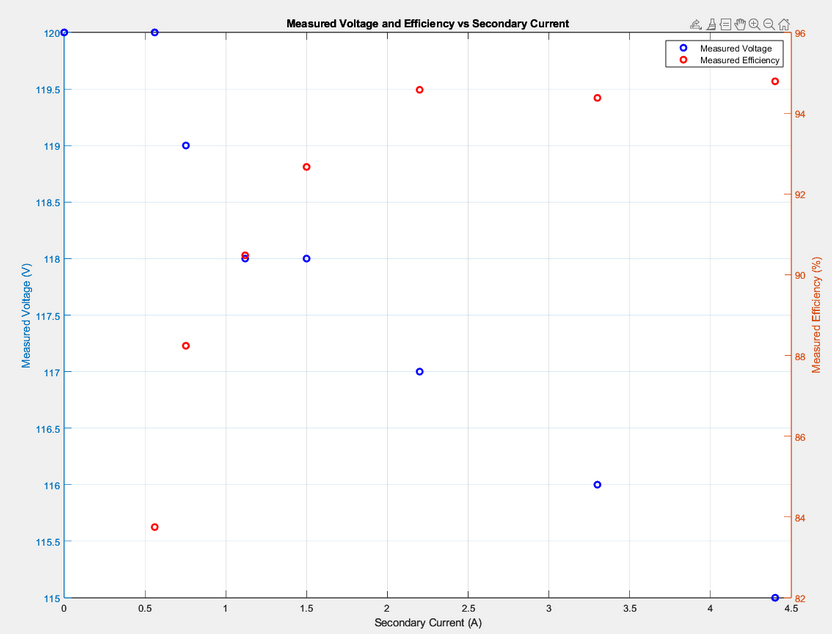
\includegraphics[width=.9\linewidth]{Screenshot 2024-09-29 at 12-34-22 Single and 3-Phase Transformers Lab 3 Report Miley Fleming 584058.docx.png}
\caption{Measured Secondary Voltage and efficiency and secondary voltage.}
\end{figure}
\end{FIGURE}

{[}Group] Compare observations with either calculated or simulated values based on your already determined equivalent circuit, by including ‘theoretical’ curves of output voltage and efficiency vs output (secondary) current on the same plots as your measured data.
\begin{FIGURE}
\begin{figure}[H]
\centering
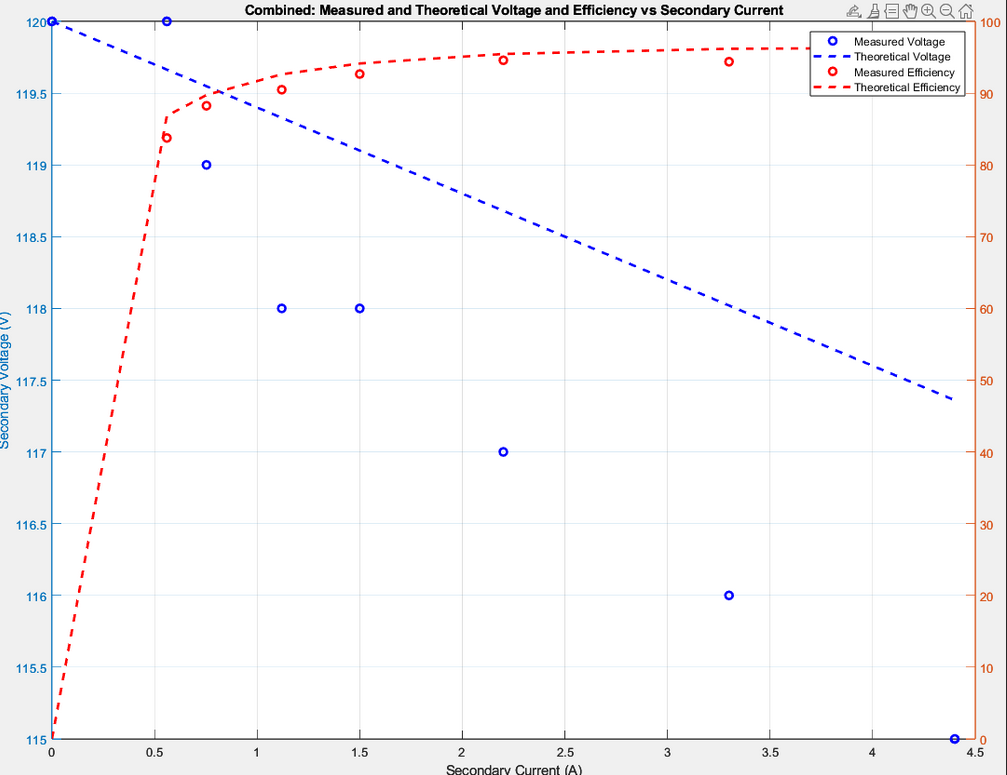
\includegraphics[width=.9\linewidth]{Screenshot 2024-09-29 at 12-36-14 Single and 3-Phase Transformers Lab 3 Report Miley Fleming 584058.docx.png}
\caption{Measured and theoretical secondary voltage and efficiency.}
\end{figure}
\end{FIGURE}
{[}Individual] Discuss generally your results, noting any major differences between observed and calculated values. Please make any other comments on your observations which you think may be interesting or relevant. \\
The voltage regulation tended to increase as the load increased, this is a measure of how well the transformer can maintain a output voltage as the load changes. Having a low voltage regulation (0\% -> 4.5\%) indicates that the transformer is able to keep a consistent voltage for a varying load. \\
The power factor initially started low and increased as the load increased, this means that the energy at low loads is not being used efficiently. As the load increased the current became more resistive and hence improved power factor.
\subsection{Three-phase Transformer Configurations}
\label{sec:org1043558}
\subsubsection{Y-Y Connected Transformer}
\label{sec:orgbed635a}
{[}Group] Present data tables showing expected and measured values for Y-Y connection.
\begin{longtable}{|l|l|l|l|l|l|l|}
\hline
 & Primary Side &  &  &  & Secondary Side & \\
\hline
\endfirsthead
\multicolumn{7}{l}{Continued from previous page} \\
\hline

 & Primary Side &  &  &  & Secondary Side &  \\

\hline
\endhead
\hline\multicolumn{7}{r}{Continued on next page} \\
\endfoot
\endlastfoot
\hline
Quantity & Expected & Observed &  & Quantity & Expected & Observed\\
\hline
VRN & 139 & 139 &  & Vrn & 139 & 139\\
\hline
VWN & 139 & 141 &  & Vwn & 139 & 142\\
\hline
VBN & 139 & 139 &  & Vbn & 139 & 139\\
\hline
VRW & 240 & 243 &  & Vrw & 240 & 243\\
\hline
VWB & 240 & 243 &  & Vwb & 240 & 243\\
\hline
VBR & 240 & 240 &  & Vbr & 240 & 240\\
\hline
\end{longtable}
\subsubsection{\(\Delta\)-Y Connected Transformer}
\label{sec:org5cd7750}
{[}Group] Present data tables showing expected and measured values for \(\Delta\)-Y connection.
\begin{longtable}{|l|l|l|l|l|l|l|}
\hline
 & Primary Side &  &  &  & Secondary Side & \\
\hline
\endfirsthead
\multicolumn{7}{l}{Continued from previous page} \\
\hline

 & Primary Side &  &  &  & Secondary Side &  \\

\hline
\endhead
\hline\multicolumn{7}{r}{Continued on next page} \\
\endfoot
\endlastfoot
\hline
Quantity & Expected & Observed &  & Quantity & Expected & Observed\\
\hline
VRW & 180 & 183 &  & Vrn & 180 & 180\\
\hline
VWB & 180 & 181 &  & Vwn & 180 & 183\\
\hline
VBR & 180 & 181 &  & Vbn & 180 & 181\\
\hline
 &  &  &  & Vrw & 311 & 315\\
\hline
 &  &  &  & Vwb & 311 & 315\\
\hline
 &  &  &  & Vbr & 311 & 320\\
\hline
\end{longtable}
\subsubsection{Y-\(\Delta\) Connected Transformer}
\label{sec:org5655e82}
{[}Group] Present data tables showing expected and measured values for Y-\(\Delta\) connection.
\begin{longtable}{|l|l|l|l|l|l|l|}
\hline
 & Primary Side &  &  &  & Secondary Side & \\
\hline
\endfirsthead
\multicolumn{7}{l}{Continued from previous page} \\
\hline

 & Primary Side &  &  &  & Secondary Side &  \\

\hline
\endhead
\hline\multicolumn{7}{r}{Continued on next page} \\
\endfoot
\endlastfoot
\hline
Quantity & Expected & Observed &  & Quantity & Expected & Observed\\
\hline
VRN & 139 & 141 &  & Vrw & 139 & 141\\
\hline
VWN & 139 & 142 &  & Vwb & 139 & 140\\
\hline
VBN & 139 & 140 &  & Vbr & 139 & 140\\
\hline
VRW & 240 & 245 &  &  &  & \\
\hline
VWB & 240 & 243 &  &  &  & \\
\hline
VBR & 240 & 242 &  &  &  & \\
\hline
\end{longtable}
\subsubsection{\(\Delta\)-\(\Delta\) Connected Transformer}
\label{sec:org9687fc6}
{[}Group] Present data tables showing expected and measured values for \(\Delta\)-\(\Delta\) connection
\begin{longtable}{|l|l|l|l|l|l|l|}
\hline
 & Primary Side &  &  &  & Secondary Side & \\
\hline
\endfirsthead
\multicolumn{7}{l}{Continued from previous page} \\
\hline

 & Primary Side &  &  &  & Secondary Side &  \\

\hline
\endhead
\hline\multicolumn{7}{r}{Continued on next page} \\
\endfoot
\endlastfoot
\hline
Quantity & Expected & Observed &  & Quantity & Expected & Observed\\
\hline
VRW & 240 & 243 &  & Vrw & 240 & 243\\
\hline
VWB & 240 & 243 &  & Vwb & 240 & 243\\
\hline
VBR & 240 & 240 &  & Vbr & 240 & 240\\
\hline
\end{longtable}
{[}Individual] Discuss your 3-phase transformer observations, noting for example the impact connection configuration has upon primary to secondary line-to-line voltage ratio, commenting on any significant differences between observed and expected voltages. \\
For each configuration we expected a voltage ratio that is some combination of \(\sqrt{3}\). The expected and observed data varied by a couple of volts, this may be because of the inaccuracies in the measuring tools and accuracy of the three-phase variac. \\
{[}Individual] Although you didn’t measure it, what else would you have expected to alter between input and output voltages, and why would that be the case? \\
The phase shift. For \(\Delta\)-Y and Y-\(\Delta\) we would expect a \(30^o\) phase shift between primary and secondary voltages. This is due to the way each of the types are connected to one another.


\newpage
\section{Bibliography}
\label{sec:orge0dba18}
Crowhurst, N. H. (2010). Waveforms when saturation occurs [Illustration]. Basic Audio. \url{http://vias.org/crowhurstba/crowhurst\_basic\_audio\_vol2\_069.html}
\newpage
\section{Appendix A}
\label{sec:org3b99799}
Code used to produce Figures 1 and 2:
\begin{center}
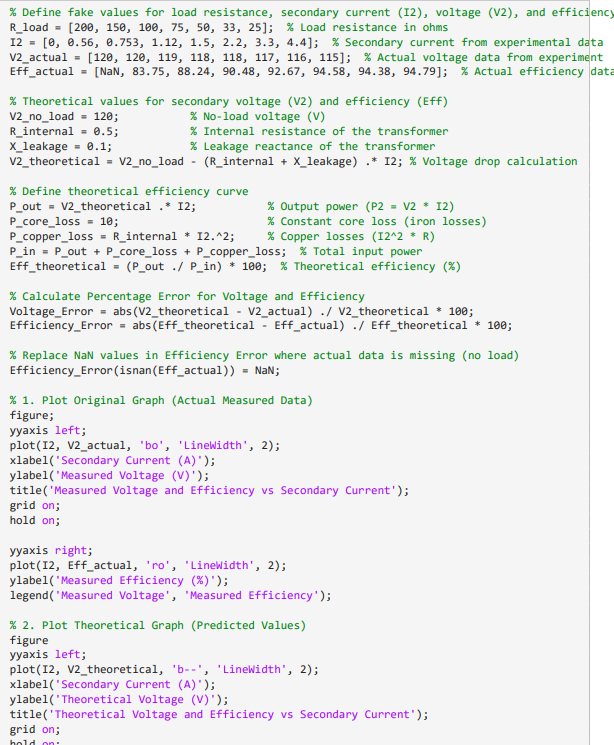
\includegraphics[width=.9\linewidth]{Code1.png}
\end{center}
\begin{center}
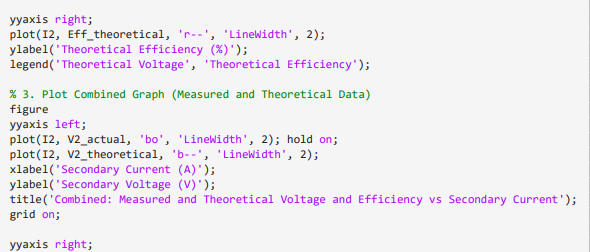
\includegraphics[width=.9\linewidth]{Code2.png}
\end{center}
\end{document}
